\documentclass[11pt]{article}
\pagestyle{empty} % Remove page number.

%%%%%%%%%%%%%%%%%%%%%%%%%%%
%%% SETUP PAGE GEOMETRY %%%
%%%%%%%%%%%%%%%%%%%%%%%%%%%
\PassOptionsToPackage{total={28cm,19cm}}{geometry} % Define the visible area when mounted inside a frame.
% \PassOptionsToPackage{showframe}{geometry} % Uncomment to show the visible area as a rectangular box.
\usepackage[a4paper,landscape]{geometry} % The frames expect A4 paper to be mounted.

%%%%%%%%%%%%%%%%%%%%%%%%%%%%
%%% SETUP IMAGE GEOMETRY %%%
%%%%%%%%%%%%%%%%%%%%%%%%%%%%
\usepackage[export]{adjustbox} % loads also graphicx
% It seems that a box with height \textheight is too large for the text body. Thus, a page break is created.
% Emperically, the following reduction was found to work. It is used when drawing the image.
\newlength{\textheightreduction}\setlength{\textheightreduction}{0.4pt}

% Correct missing options for \includegraphics that was removed with TeXLive 2016 onwards.
% See https://tex.stackexchange.com/a/407167/25523 and https://tex.stackexchange.com/a/392679/25523.
\makeatletter
\define@key{Gin}{resolution}{\pdfimageresolution=#1\relax}
\makeatother

%%%%%%%%%%%%%%%%%%%%%%%%%%%%%%%%%%%
%%% SETUP DRAWING FUNCTIONALITY %%%
%%%%%%%%%%%%%%%%%%%%%%%%%%%%%%%%%%%
\usepackage[usenames,dvipsnames]{xcolor}
\usepackage{tikz}
\usetikzlibrary{patterns}

%%%%%%%%%%%%%%%%%%%%%%%%%
%%% USE ACM TOG FONTS %%%
%%%%%%%%%%%%%%%%%%%%%%%%%
\usepackage[tt=false, type1=true]{libertine}
\usepackage[varqu]{zi4}
\usepackage[libertine]{newtxmath}
\usepackage[T1]{fontenc}

%%%%%%%%%%%%%%%%%%%%
%%% SETUP COLORS %%%
%%%%%%%%%%%%%%%%%%%%
\colorlet{BackgroundColor}{black} % Be sure that your image background is exactly this color. Do a test print.
\colorlet{TextboxColor}{black} % The color of the box around the text.
\colorlet{TextColor}{white} % The color of the text itself.
% Consult https://en.wikibooks.org/wiki/LaTeX/Colors on named colors and on how to define your own colors.
% In case any of the following colors is not needed (i.e., the corresponding element is transparent), then
%  set an arbitrary color (e.g., black) and use 'opacity=0' or 'text opacity=0' in the TikZ commands below.

%%%%%%%%%%%%%%%%
%%% DOCUMENT %%%
%%%%%%%%%%%%%%%%
\begin{document}
	\noindent % Prevent indentation before image.
	%
	% Draw background color over the whole page.
	\begin{tikzpicture}[remember picture,overlay]
		% There are two options for setting the background color:
		%   1.) Using a vector graphic rectangle, which is filled with the background color; or
		%   2.) Using a part of the image that is stretched over the whole page.
		% For the first option, just uncomment the following command:
%        \draw[fill=BackgroundColor] (current page.south east) rectangle (current page.north west);
		%
		% However, it can be hard to exactly match the background color of the image and the LaTeX provided colors.
		% Especially a pure black background can be problemantic as PDF and printer driver interpret 'black' in
		%  different ways. See https://graphicdesign.stackexchange.com/a/2999 for details.
		% In this case it is preferable to just take a cropped version of the actual image as background. For this,
		%  uncomment the command below and set the 'resolution=' to the DPI resolution of the image. Furthermore,
		%  specify a region of the image, which should ONLY contain the background color, via the 'viewport='
		%  command. The origin of the viewport is the lower left corner of the image.
		\node[inner sep=0pt,anchor=north west]
			at (current page.north west)
			{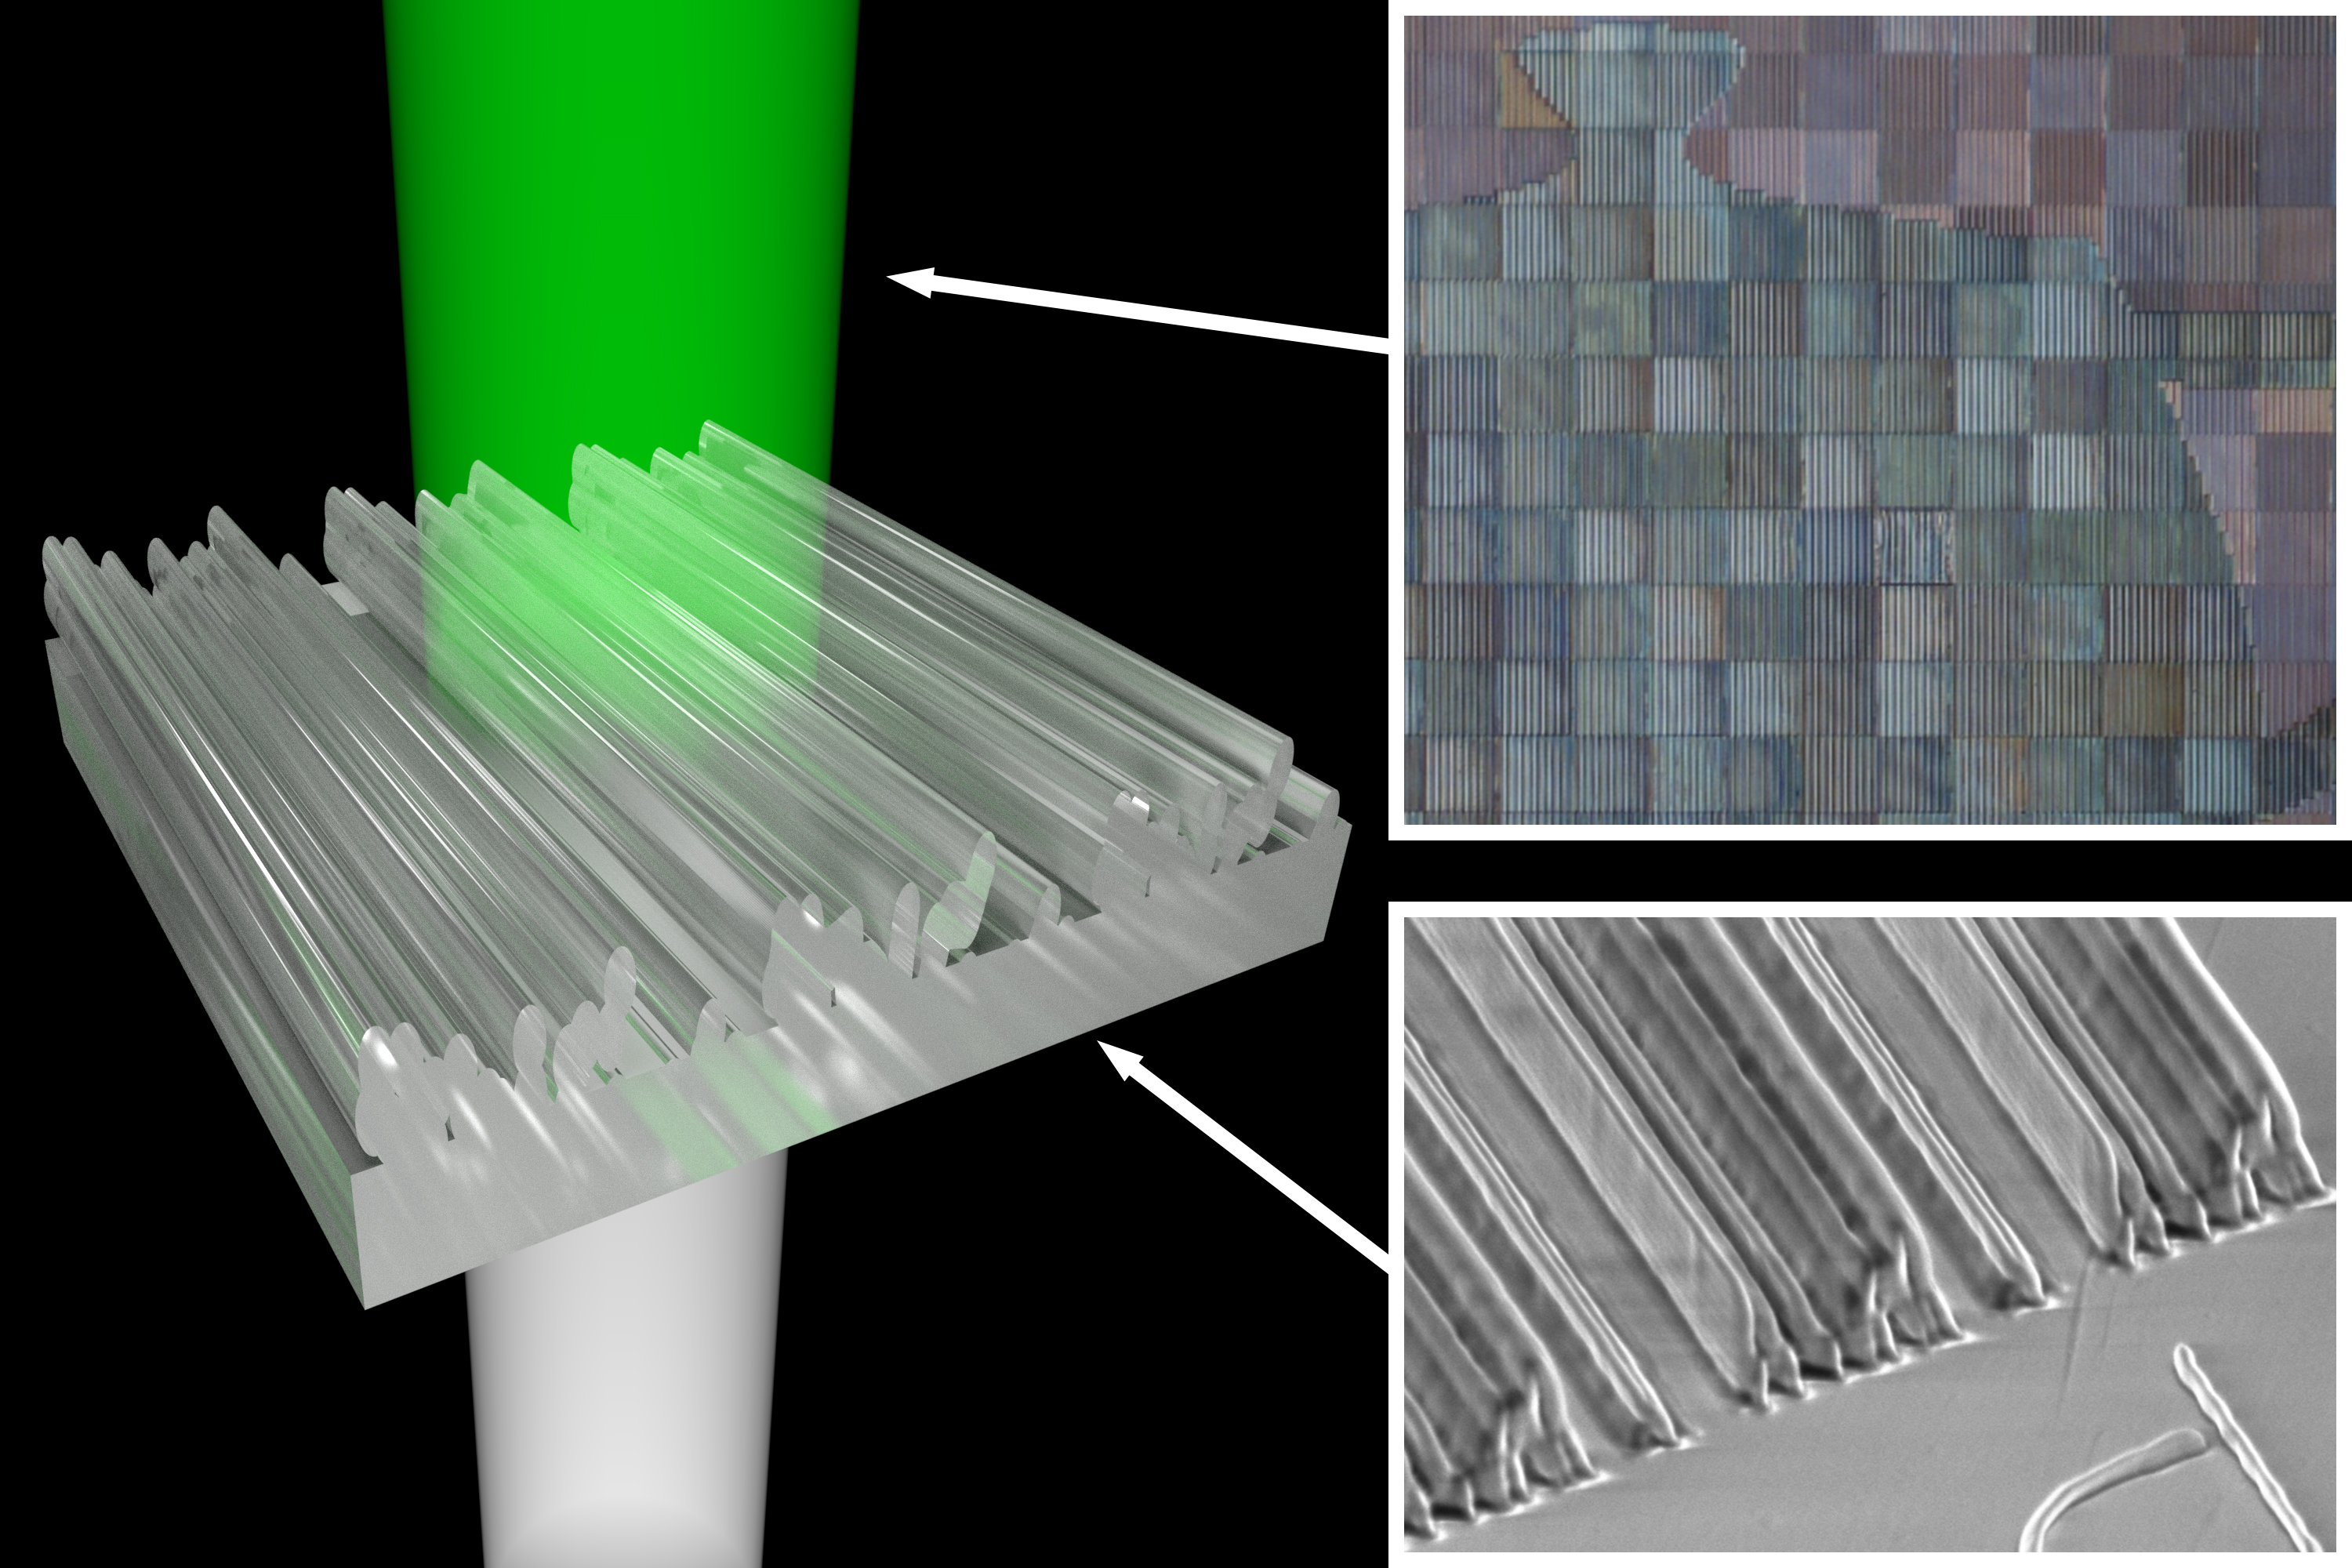
\includegraphics[
				resolution=72,viewport=0px 0px 64px 64px,clip,
				width=\paperwidth,height=\paperheight]{image}};
		% Idealy, one would just use a single background pixel from the image. However, the above command can fail for
		%  an image region smaller than 64 by 64 pixel on Linux (and up to 256 by 256 pixel on Windows).
		% If this is a problem, a (single-pixel) background image needs to explicitly generated outside of LaTeX.
	\end{tikzpicture}
	%
	% Draw image and accompanying text. Keep the default font values to ensure uniformity of the gallery.
	\begin{tikzpicture}
		% Draw the image. Possible alignments are:
		%   *) Centered: Use 'anchor=north'      and 'at (0.5\textwidth,...)'.
		%   *) Left:     Use 'anchor=north west' and 'at (0,...)'.
		%   *) Right:    Use 'anchor=north east' and 'at (\textwidth,...)'.
		% To verically center the image use 'inner ysep=Xcm' where X is a suitable number. Generally, this is only
		%  necessary if the image width is significantly larger than its height.
		\node[inner xsep=0pt, inner ysep=0cm,anchor=north]
			at (0.5\textwidth,\textheight-\textheightreduction)
			% For the 'max height' below, use a scaled value of the \textheight so that your image is as large as
			%  possible without colliding with the text box.
			{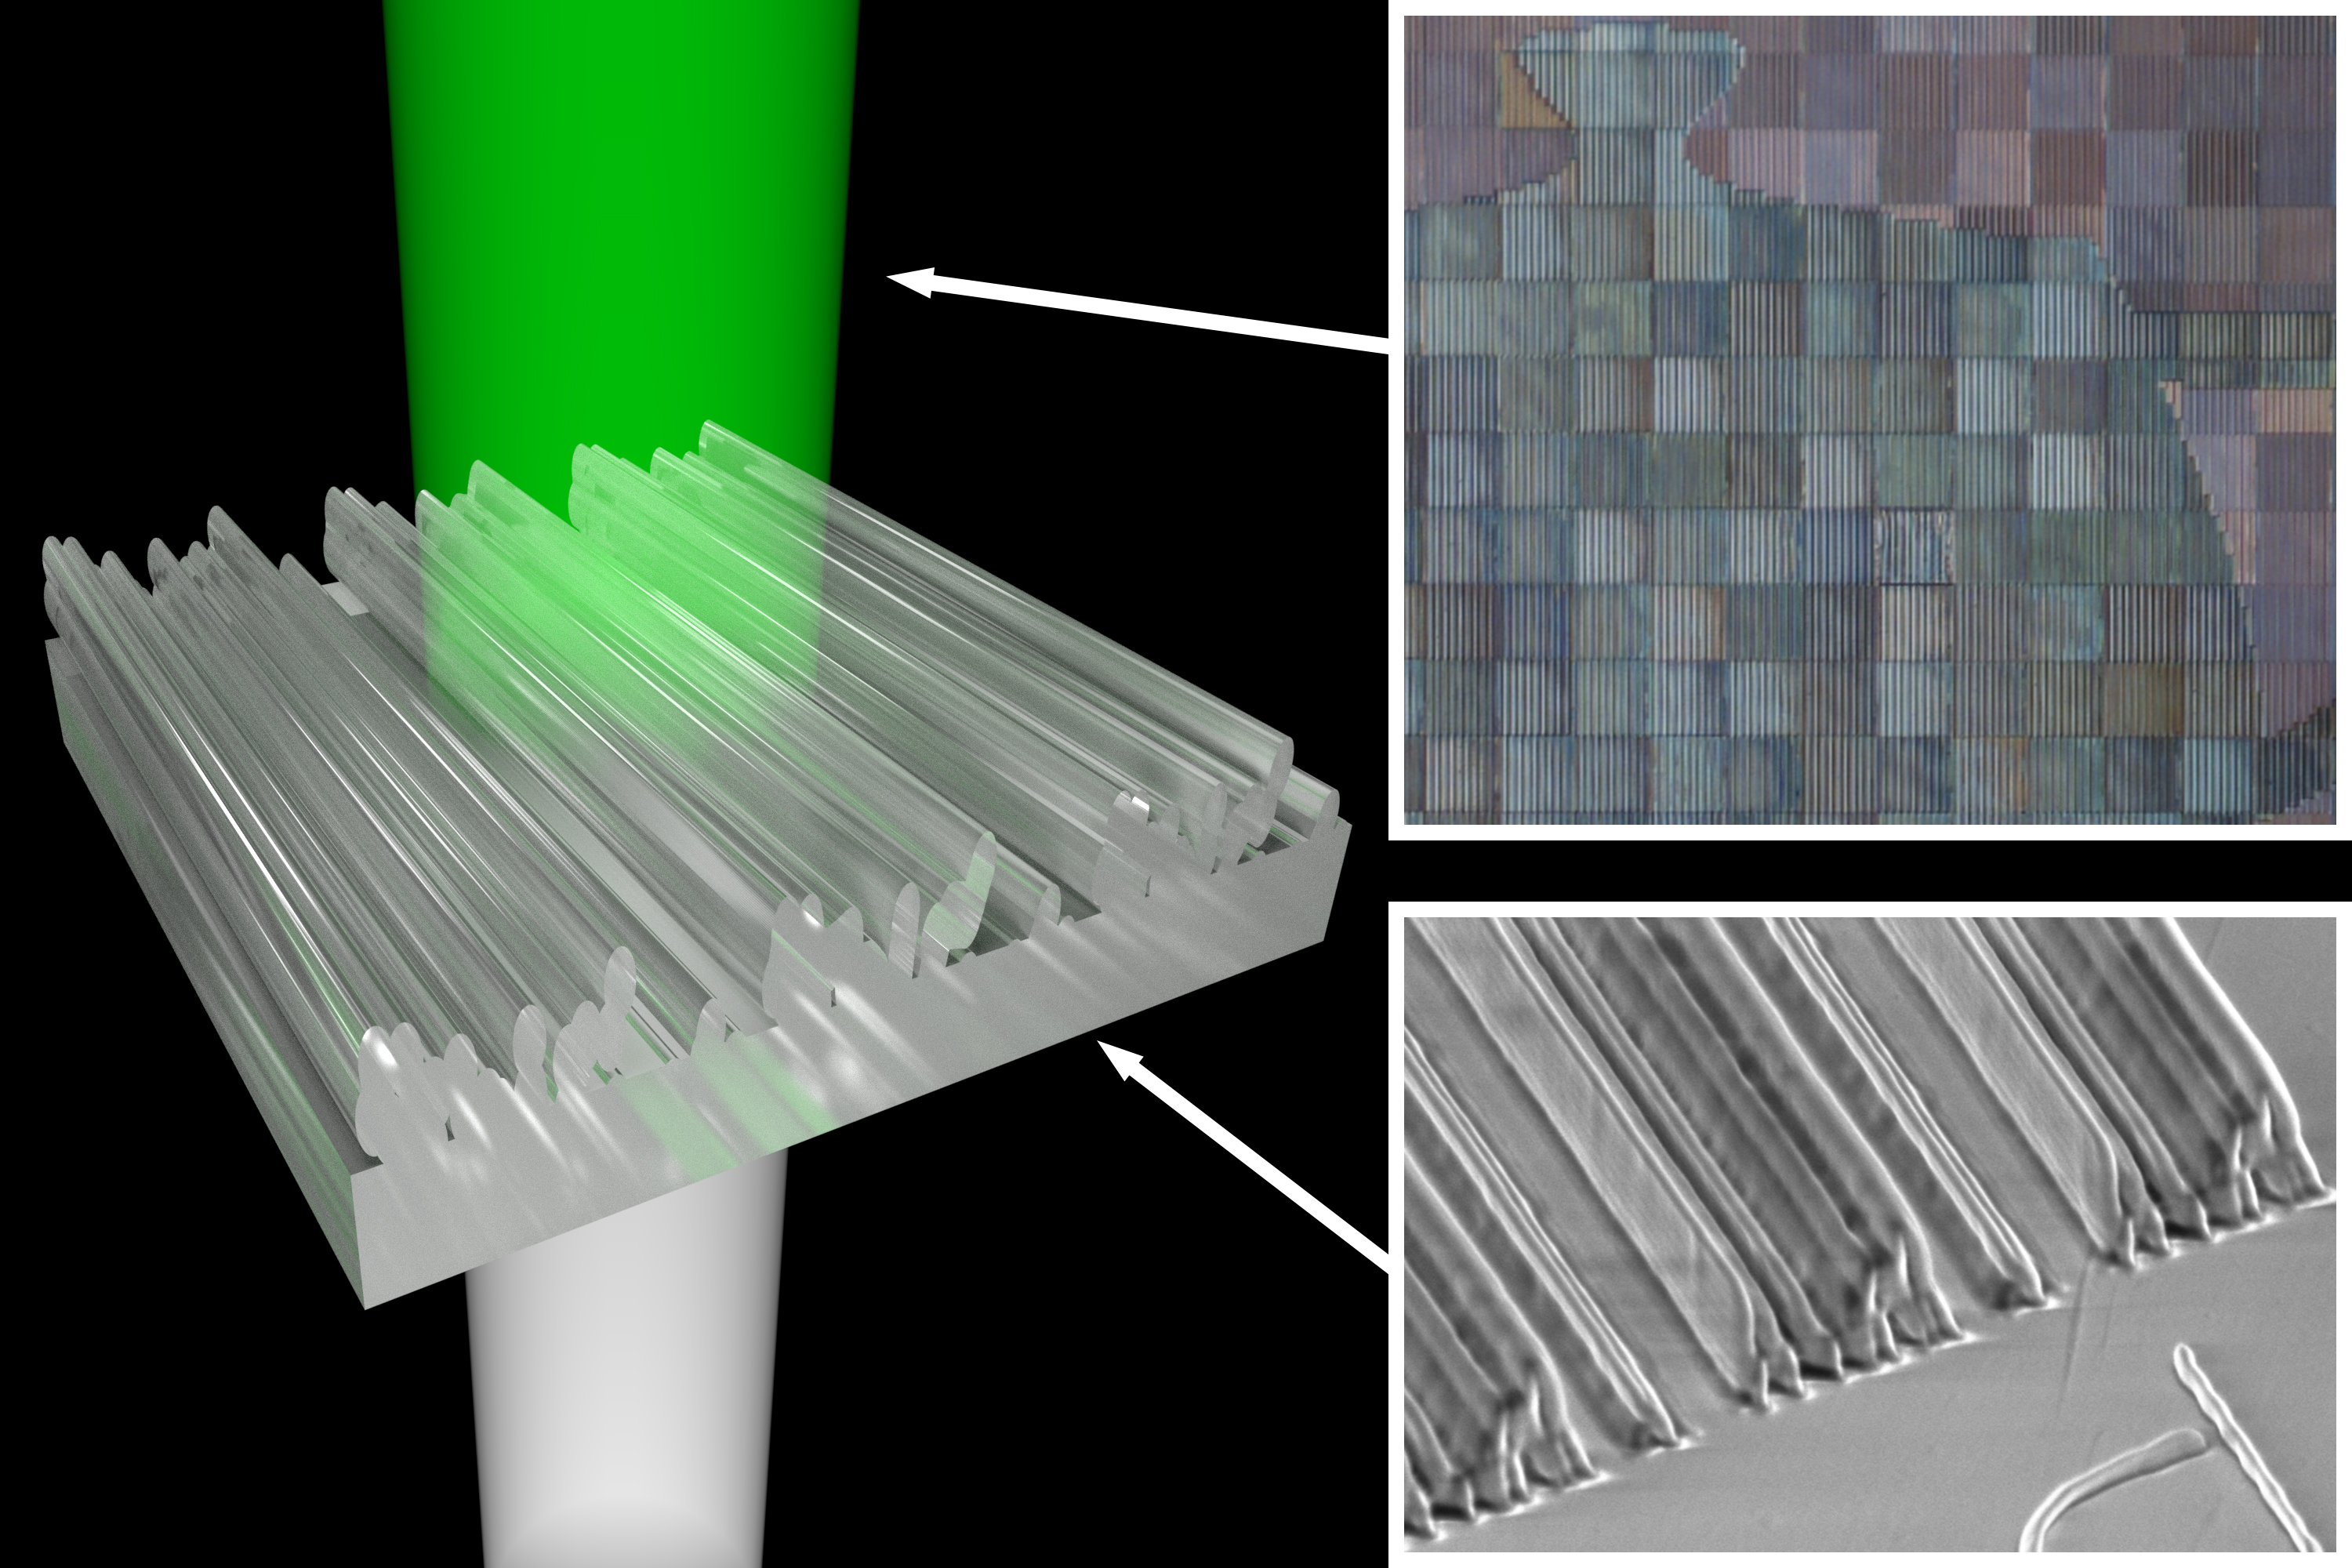
\includegraphics[max width=\textwidth,max height=.67\textheight]{image}};
		%
		% Draw the text box. Use the 'opacity' value to make the textbox (partially) transparent.
		\node[fill=TextboxColor,opacity=0,text opacity=1,text=TextColor,
			anchor=south west,align=left,text width=\textwidth]
		at (0,0) % The origin is placed at the lower left corner of the page's text body.
		{
			\medskip

			% Add a title.
			{\LARGE\textbf{Computational Design of Nanostructural Color for Additive Manufacturing}}
			\bigskip

			% Add the authors. IST Austria members optionally in bold. Affiliations as superscript numbers.
			{\large\textbf{Thomas AUZINGER}${}^1$, Wolfgang HEIDRICH${}^2$, \textbf{Bernd BICKEL}${}^1$}
			\hfill
			% Add the affiliations. Again use superscript numbers.
			{\large ${}^1$IST Austria \quad ${}^2$KAUST}
			\medskip

			% Add the publication venue.
			{\large\textbf{ACM Transactions on Graphics 37(4) (SIGGRAPH 2018)}}
			\medskip

			% Add a description of the work (e.g., the paper abstract).
			% Keep this a short as possible; the image should dominate the final result!
			{\small Additive manufacturing has recently seen drastic improvements in resolution, making it now possible to fabricate features at scales of hundreds or even dozens of nanometers, which previously required very expensive lithographic methods.
			As a result, additive manufacturing now seems poised for optical applications, including those relevant to computer graphics, such as material design, as well as display and imaging applications.
			% Avoid line breaks in the abstract text to shorten it.
			In this work, we explore the use of additive manufacturing for generating structural colors, where the structures are designed using a fabrication-aware optimization process.
			This requires a combination of full-wave simulation, a feasible parameterization of the design space, and a tailored optimization procedure.
			Many of these components should be re-usable for the design of other optical structures at this scale.
			% Avoid line breaks in the abstract text to shorten it.
			We show initial results of material samples fabricated based on our designs.
			While these suffer from the prototype character of state-of-the-art fabrication hardware, we believe they clearly demonstrate the potential of additive nanofabrication for structural colors and other graphics applications.}
		};
	\end{tikzpicture}
\end{document}
